\documentclass{article}

%% Packages %%

\usepackage{layout}
\usepackage{xcolor}
\usepackage{amsfonts}
\usepackage{hyperref}
\usepackage{setspace}
\hypersetup{
  colorlinks=true,
  linkcolor=black,
  filecolor=black!5,
  urlcolor=black,
  pdftitle={Vernon Grant},
  pdfpagemode=FullScreen,
}
\usepackage[a4paper,top=1cm,bottom=1cm,left=1.5cm,right=1.5cm]{geometry}

%% Document Margins %%

\marginparwidth 0pt
\marginparsep 0pt

%% Tikz %%

\usepackage{tikz}
\usetikzlibrary{patterns}
\usetikzlibrary {arrows.meta}

%% Global Variables %%

\newcommand{\DiagramMaxWidth}{18cm}

\newcommand{\ExternalLink}{%
  \tikz[x=1.2ex, y=1.2ex, baseline=-0.05ex]{%
    \begin{scope}[x=1ex, y=1ex]
      \clip (-0.1,-0.1)
      --++ (-0, 1.2)
      --++ (0.6, 0)
      --++ (0, -0.6)
      --++ (0.6, 0)
      --++ (0, -1);
      \path[draw,
        line width = 0.5,
        rounded corners=0.5]
      (0,0) rectangle (1,1);
    \end{scope}
    \path[draw, line width = 0.5] (0.5, 0.5)
    -- (1, 1);
    \path[draw, line width = 0.5] (0.6, 1)
    -- (1, 1) -- (1, 0.6);
  }
}

% Document:
\begin{document}

%% ------------------- %%
%% Introduction Header %%
%% ------------------- %%

\noindent
\begin{tikzpicture}[fill=white]
  %% Outer rectangle
  \draw[anchor=north west, color=black] (0,0) rectangle (18,3);

  %% Profile photo
  \node[inner sep=0pt, anchor=north west] (Vernon Grant) at (0,3)
       {
\includegraphics[width=2.9855cm]{profile.jpg}};
       \draw (3.43,2.4) node[anchor=north west] (a) {\Huge Vernon Grant};
       \draw (4.35,1.35) node[text=black!50, anchor=north west] (b) {\Large {\emph {Web Developer}}};

       %% Social media
       \draw[fill=white] (9,3) rectangle (13,2) node[pos=.5] {\href{https://github.com/VernonGrant}{\ExternalLink GitHub}};
       \draw[fill=white] (9,2) rectangle (13,1) node[pos=.5] {\href{https://vernon-grant.com/}{\ExternalLink Blog}};
       \draw[fill=white] (9,1) rectangle (13,0) node[pos=.5] {\href{https://twitter.com/home}{\ExternalLink Twitter}};

       %% Contact details
       \draw (13,3) rectangle (18,2) node[pos=.5] {vernon@ruppell.io};
       \draw (13,2) rectangle (18,1) node[pos=.5] {+270 0000 0000};
       \draw (13,1) rectangle (18,0) node[pos=.5] {Cape Town, South Africa};
\end{tikzpicture}
\break

%% ----------------- %%
%% Summary Statement %%
%% ----------------- %%

\noindent

\begin{tikzpicture}[fill=white]
  \draw (0,0) rectangle (9,1) node at (4.5,.5) {\large Summary Statement};
  \draw[color=black] (9,0.5) -- (18,0.5);
\end{tikzpicture}

\vspace{0.5cm}
\noindent I am an South African Web Developer with over five years of experience working in Hong Kong. I have developed expertise across various programming languages such as PHP, JavaScript, C, Clojure and more. I'm a very fast learner and enjoy coming up with simple and maintainable solutions to problems. While also having a keen eye for business analysis and problem-solving abilities that make me an asset to any company or organization looking to expand their digital footprint.
\vspace{0.65cm}

%% ---------- %%
%% Experience %%
%% ---------- %%

\noindent

\begin{tikzpicture}[fill=white]
  \draw (0,0) rectangle (9,1) node at (4.5,.5) {\large Professional Experience};
  \draw[color=black] (9,0.5) -- (18,0.5);
\end{tikzpicture}

% Full-Stack Web Developer
\vspace{0.5cm}

\begin{doublespace}
  \noindent {\Large Full-Stack Web Developer} \newline
  \noindent {\large \href{https://ruppell.io/en-hk/}{\ExternalLink Ruppell Limited} | 2018 - Current \hfill \emph{Hong Kong}}
\end{doublespace}
\noindent I was responsible for developing both frontend (client-side scripting) as well as backend (server-side programming) solutions. I had to make use of various frameworks and languages such as Electron, Flutter, Bash, C, JavaScript, PHP, Clojure and more. I also managed virtual servers by updating SSL certificates, extracting statistical data from databases and keeping general security and backups up to date.

% Web Developer
\vspace{0.5cm}
\begin{doublespace}
  \noindent {\Large Web Developer} \newline
  \noindent {\large \href{https://3trinity.hk/en-hk/home/}{\ExternalLink Trinity International Limited}  | 2015 - 2018 \hfill \emph{Hong Kong}}
\end{doublespace}
\noindent I was responsible for creating and maintaining websites by using various programming languages such as HTML, CSS, JavaScript and PHP. I was expected to design user-friendly interfaces that can be easily navigated through on mobile, tablet and desktop devices. Apart from this I had to make use of SEO (Search Engine Optimization) techniques to help improve the visibility and ranking of the companies websites online.
\vspace{0.5cm}

% General Office Administrator
\begin{doublespace}
  \noindent {\Large General Office Administrator} \newline
  \noindent {\large \href{https://www.seedland.hk}{\ExternalLink Seedland International Limited} | 2010 - 2015 \hfill \emph{Hong Kong}}
\end{doublespace}
\noindent As general office administrator, I was responsible for managing and coordinating various administrative tasks within the company, such as answering phones, greeting visitors, handling mail, scheduling appointments, maintaining filing systems, organizing meetings, arranging travel plans, preparing reports, processing expense claims, overseeing office supplies and inventory management.

\vspace{0.65cm}

%% --------------- %%
%% Recent Projects %%
%% --------------- %%

\noindent

\begin{tikzpicture}[fill=white]
  \draw (0,0) rectangle (9,1) node at (4.5,.5) {\large Recent Projects};
  \draw[color=black] (9,0.5) -- (18,0.5);
\end{tikzpicture}
\break

% Discovering Emacs
\begin{doublespace}
  \noindent {\Large \href{https://github.com/VernonGrant/discovering-emacs}{\ExternalLink Discovering Emacs} \hfill \emph{Lisp}}
\end{doublespace}
\noindent Educational content all about GNU Emacs, where I uncover some of its lesser known features, discussed upcoming releases and share some tips and tricks. Join me as we discover some of the most valuable aspects of this wonderful piece of software.
\vspace{0.5cm}

\pagebreak

% GNU C Language Manual
\begin{doublespace}
  \noindent {\Large \href{https://github.com/VernonGrant/gnu-c-language-manual}{\ExternalLink GNU C Language Manual} \hfill \emph{C, Bash}}
\end{doublespace}
\noindent I developed a series of custom C utilities and shell scripts to convert \textbf{Richard Stallman's} new GNU C Language Intro and Reference Manual to Markdown. I also contributed to the manual by communicating directly with Richard, pointing out any mistakes or issues I've found.
\vspace{0.5cm}

% Sidekick.el
\begin{doublespace}
  \noindent {\Large \href{https://github.com/VernonGrant/sidekick.el}{\ExternalLink Sidekick.el} \hfill \emph{Lisp, Bash, Emacs}}
\end{doublespace}
\noindent Sidekick is an Emacs package that's aim is to provide information about a symbol inside a single window. It's still in its infancy, and at this point in time only searches for references using ripgrep. It will however be in active development and I hope to extend it in the near future to support things such as getting a symbols documentation and extracting other time saving information.
\vspace{0.5cm}

% Abbreviate.el
\begin{doublespace}
  \noindent {\Large \href{https://github.com/VernonGrant/abbreviate.el}{\ExternalLink Abbreviate.el} \hfill \emph{Lisp, Emacs}}
\end{doublespace}
\noindent Abbreviates the word at point, using a predefined list of common programming abbreviations. I made this package because I always forget certain abbreviations, and the abbreviations I use are inconsistent across code bases.
\vspace{0.5cm}

% Json.c
\begin{doublespace}
  \noindent {\Large \href{https://github.com/VernonGrant/jsn.c}{\ExternalLink JSN.c} \hfill \emph{C, JSON, Make, Bash}}
\end{doublespace}
\noindent A C JSON utility developed from scratch that's intended to be used for parsing, generating and manipulating JSON files.
\vspace{0.65cm}

%% ---------------- %%
%% Higher Education %%
%% ---------------- %%

\noindent

\begin{tikzpicture}[fill=white]
  \draw (0,0) rectangle (9,1) node at (4.5,.5) {\large Higher Education};
  \draw[color=black] (9,0.5) -- (18,0.5);
\end{tikzpicture}

\vspace{0.5cm}
\begin{doublespace}
  \noindent {\Large Diploma in Information and Communications Technologies} \newline
  \noindent {\large \href{https://welkin.com.hk}{\ExternalLink Welkin Systems Limited} | 2013 \hfill \emph{Hong Kong}}
\end{doublespace}

\noindent I completed a Diploma that covered various protocols and technologies that make up the Internet, such as HTTP (Hypertext Transfer Protocol), TCP/IP (Transmission Control Protocol /Internet Protocol) , DNS (Domain Name System), FTP (File Transfer Protocol). Also included fundamental HTML, CSS and JavaScript topics. \newline
\vspace{0.65cm}

%% ------ %%
%% Skills %%
%% ------ %%

\noindent

\begin{tikzpicture}[fill=white]
  \draw (0,0) rectangle (9,1) node at (4.5,.5) {\large Experienced In};
  \draw[color=black] (9,0.5) -- (18,0.5);
\end{tikzpicture}
\break

\noindent
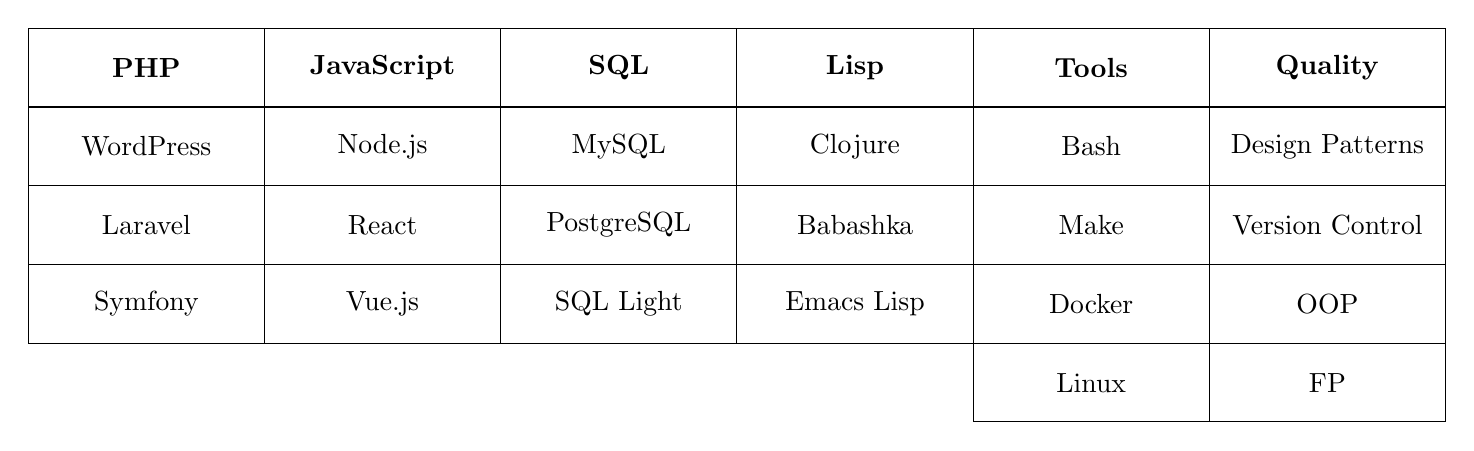
\begin{tikzpicture}[fill=white]
  \draw[anchor=north west, color=black] (0,0) rectangle (18,3);

  \draw[fill=white] (0,3) rectangle (3,2) node[pos=.5] {\textbf{PHP}};
  \draw[fill=white] (0,2) rectangle (3,1) node[pos=.5] {WordPress};
  \draw[fill=white] (0,1) rectangle (3,0) node[pos=.5] {Laravel};
  \draw[fill=white] (0,0) rectangle (3,-1) node[pos=.5] {Symfony};

  \draw[fill=white] (3,3) rectangle (6,2) node[pos=.5] {\textbf{JavaScript}};
  \draw[fill=white] (3,2) rectangle (6,1) node[pos=.5] {Node.js};
  \draw[fill=white] (3,1) rectangle (6,0) node[pos=.5] {React};
  \draw[fill=white] (3,0) rectangle (6,-1) node[pos=.5] {Vue.js};

  \draw[fill=white] (6,3) rectangle (9,2) node[pos=.5] {\textbf{SQL}};
  \draw[fill=white] (6,2) rectangle (9,1) node[pos=.5] {MySQL};
  \draw[fill=white] (6,1) rectangle (9,0) node[pos=.5] {PostgreSQL};
  \draw[fill=white] (6,0) rectangle (9,-1) node[pos=.5] {SQL Light};

  \draw[fill=white] (9,3) rectangle (12,2) node[pos=.5] {\textbf{Lisp}};
  \draw[fill=white] (9,2) rectangle (12,1) node[pos=.5] {Clojure};
  \draw[fill=white] (9,1) rectangle (12,0) node[pos=.5] {Babashka};
  \draw[fill=white] (9,0) rectangle (12,-1) node[pos=.5] {Emacs Lisp};

  \draw[fill=white] (12,3) rectangle (15,2) node[pos=.5] {\textbf{Tools}};
  \draw[fill=white] (12,2) rectangle (15,1) node[pos=.5] {Bash};
  \draw[fill=white] (12,1) rectangle (15,0) node[pos=.5] {Make};
  \draw[fill=white] (12,0) rectangle (15,-1) node[pos=.5] {Docker};
  \draw[fill=white] (12,-1) rectangle (15,-2) node[pos=.5] {Linux};

  \draw[fill=white] (15,3) rectangle (18,2) node[pos=.5] {\textbf{Quality}};
  \draw[fill=white] (15,2) rectangle (18,1) node[pos=.5] {Design Patterns};
  \draw[fill=white] (15,1) rectangle (18,0) node[pos=.5] {Version Control};
  \draw[fill=white] (15,0) rectangle (18,-1) node[pos=.5] {OOP};
  \draw[fill=white] (15,-1) rectangle (18,-2) node[pos=.5] {FP};
\end{tikzpicture}
\end{document}
